\section{Answer part one}
%Identify the stakeholders in your project and describe their interests in the project and  how you will handle them
\begin{center}
	\begin{tabular}[h]{|c|p{25em}|}
		\hline
		Stakeholder & Interest \\ \hline
		General Practitioners & They are our target demographic as they use the service to provide better healthcare to their clients. Developing our program will be able to increase the confidence of their diagnoses. \\ \hline
		Developers & They are interested in it because their business and thereby wages depends on it, delivering a good product could gain them good advantages when it comes to income and or future job prospects. \\ \hline
		Healthcare companies & The companies that hires the General Practitioners are the one who will most likely be paying for our service, their interested is whether this will earn them more revenue either in the long run or short term.\\ \hline
	\end{tabular}
\end{center}

%Create a WBS for your project and document it as a table
In this project, the group are using a Top-Down estimation process because of the following reasons:
\begin{itemize}
	\item It's the first time the group develops a project for healthcare and thereby don't know completely what is involved yet.
	\item It's a small project and the group only have two developers, the scope of the project is small.
	\item There is no contract involved.
	\item There is no current customer, only general practitioners who have offered to guide and therefore no details are needed for the customers.
\end{itemize}
For the development of the product, it is split up in 3 section in the WBS, Frontend, Backend and server. 
\begin{center}
	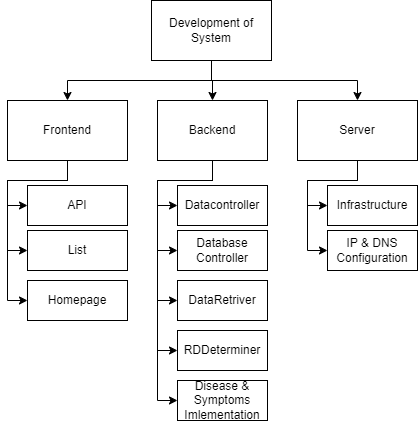
\includegraphics[width=.5\columnwidth]{./WBS}
\end{center}

\begin{center}
	\begin{tabular}[h]{|c|c|c|}
		\hline
		Task & Dependency & Estimated Time (hours) \\ \hline
		ISymptom & & \\ \hline
		Region & &  \\ \hline
		IDisease & &  \\ \hline
		Symptom & ISymptom, Region &  \\ \hline
		Disease & IDisease & \\ \hline
		DatabaseController & Disease, Symptom & \\ \hline
		DataController & DatabaseController &  \\ \hline
		DataRetriver & DatabaseController & \\ \hline
		IDeterminer & &  \\ \hline
		RDDeterminer & IDeterminer, DataRetriver & \\ \hline
		API & DataController & \\ \hline
		Homepage & & \\ \hline
		Infrastructure & & \\ \hline
		IP \& DNS & Homepage & \\ \hline
	\end{tabular}
\end{center}

Slut: 28.April
%Write a POS for your project using the template on p. 126 in Effective Project Management(Wysocki)
\begin{center}
	\begin{tabular}[h]{|p{7em}|p{5em}|p{5em}|p{5em}|p{5em}|}
		\hline
		& {\scriptsize Project Overview Statement} & {\scriptsize Rare disease Predictor} & & {\scriptsize Simon dos Reis Spedsbjerg} \\ \hline
		{\scriptsize Problem/Opportunity} & \multicolumn{4}{|p{20em}|}{\scriptsize We see a risk that a healthcare professional might miss certain rare conditions a patient might suffer from, because the rarity and lack of knowledge makes it so the doctor or nurse might not suspect it and thereby miss it.}\\ \hline
		{\scriptsize Goal} & \multicolumn{4}{|p{20em}|}{\scriptsize To develop an application that will help the health care professional to deduce whether a patient suffers from a rare disease}\\ \hline
		{\scriptsize Objectives} & \multicolumn{4}{|p{20em}|}{\scriptsize \begin{itemize}
		\item Develop a Backend system to calculate diseases based on symptoms
		\item Develop a Frontend to allow interaction from any computer
		\item Establish a server to host a beta version
		\item Deploy public version
			 \end{itemize}
		 } \\ \hline
	 {\scriptsize Success Criteria} & \multicolumn{4}{|p{20em}|}{\scriptsize\begin{itemize}
	 	\item The system can predict diseases based on given symptoms
	 	\item The system is positively received by general practitioners
	 	\item The system is being used by general practitioners
	 \end{itemize}} \\ \hline
 	{\scriptsize Assumptions, Risks, Obstacles} & \multicolumn{4}{|p{20em}|}{\scriptsize
 	\begin{itemize}
 		\item All general practitioners have access to the internet
 		\item Server Errors might occur
 		\item Some general practitioners don't have the required computer knowledge to use the system
 	\end{itemize}	
 }\\ \hline
& {\scriptsize Simon Spedsbjerg} & {\scriptsize $07-03-23$} & & \\ \hline
	\end{tabular}
\end{center}
%Identify the risks in the project, create a risk severity matrix, and explain how you will handle the risks
\begin{center}
	\centering
	\begin{tabular}[h]{|p{4em}|p{6em}|p{6em}|p{6em}|p{6em}|p{6em}|}
		\hline
		Very High (71-90\%)  &  Healthcare tech companies do not want to add the product to their catalogue of software. &         The development team is composed of students meaning there is a general inexperience for developing. & & &                                                                     \\ \hline                                                                                                                                                                                                                                                
		High   (51-70\%)   & & & Lack of knowledge in the field area could lead to a worse quality product & & \\ \hline
		Medium (31-50\%)  & & Some general practitioners might not have the computer knowledge to use the system. & The lack of data for diseases and symptoms. & Since it is new territory to develop medical based software, there might be certain elements we do not know of that would add elements out of scope & \\ \hline
		Low   (11-30\%)   & & & & & \\ \hline
		Very Low (<10\%) & The algorithm could produce a faulty result. & & GP’s might not use the product due to it not being on their main system. & The servers can go down leading to down time. & \\ \hline
		Likelihood / Impact & Very Low & Low & Medium & High & Very High \\ \hline
	\end{tabular}
\end{center} 
\pagebreak
There are ways to combat some of the risks involved in the project, but some of them are risks we must accept comes with the creation of the product.

\begin{itemize}
	\item For the risks involving the usage of the product and problems possibly arising with it, it would be possible to try and avoid that risk with the creation of a better user interface to make it easier for GP’s who does not have a lot of general computer knowledge. 
	\item For the risks involving inexperience with the medical software field, the only way to try combat it, would be to try and overestimate how much time it will take to develop and create the system, that way it would allow the team more time than normal to complete the system, and it would not cause any issues for the stakeholders, due to going over the planned time and possibly even finishing earlier than the planned time given.
	\item The risk involving the actual system and algorithm, the risk can be reduced if not removed by creating multiple tests to try and break the algorithm. If the algorithm passes the tests, the risk should not have an effect.
	\item For the risks of having the servers go down, that is something we have to accept that is always a possibility that can happen for any system, the only way to reduce the chances for this to happen, would be to choose a reliable server host which has the least amount of downtime over a longer period.
	\item For the risk involving the lack of data, a way to avoid it making or breaking the system would be to create dummy data in its place, if the data is not acquired. Granted this will end up with a result that cannot be practically used, it would end up with a system that can showcase the functionality required of it, and it would be a simple case of swapping around data sets.
	\item For the Health companies not adding it to their system or GP’s not wanting to use it if its not on their system is another risk we just must accept. It is not in our hands if the company does not want to add it nor if the GPs don’t want to use anything outside their known toolbox.
\end{itemize}

%Estimate the tasks in your WBS. Argue for the selection of estimation method

%Create a network diagram for your project and identify 1) the earliest finish date for theproject and 2) the critical path
\pagebreak
\begin{figure}
	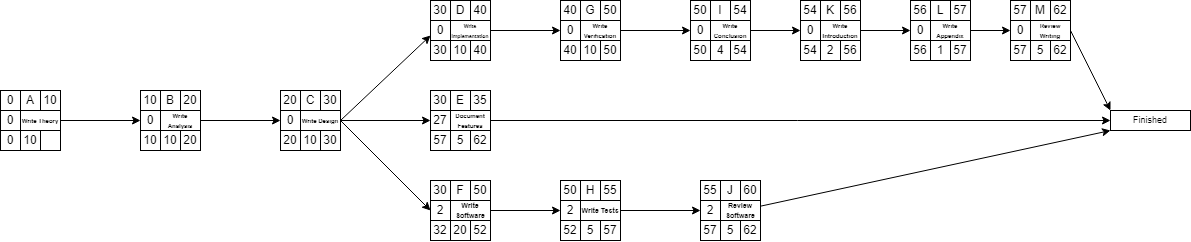
\includegraphics[width=40em,keepaspectratio]{Network Diagram.png}
\end{figure}

The diagram above is a network diagram created in the node style for the project. All the timeframes are approx. estimations we assumed how long each part would take. This network diagram is created with the entire bachelor as a project, where report writing creating the software and anything else required is included.

\begin{itemize}
	\item The earliest finish date based on the network diagram would take 62 calendar units.
	\item The critical path in this network diagram is the following sequence.
	\begin{itemize}
		\item A->B->C->D->G->I->K->L->M
	\end{itemize}
\end{itemize}
%Create  a  short  presentation  that  you  can  use  in  class  to  present  your  results  to  othergroups


Read stuff from\cite{Larson2021}.